\documentclass[ALICE,manyauthors]{ALICE_analysis_notes}
%\documentclass[ALICE,manyauthors]{ALICE_scientific_notes}
%
%\newcommand{\jpsi}{\rm J/$\psi$}
%\newcommand{\psip}{$\psi^\prime$}
%\newcommand{\jpsiDY}{\rm J/$\psi$\,/\,DY}
%\newcommand{\dd}{\mathrm{d}}
%\newcommand{\chic}{$\chi_{\rm c}$}
%\newcommand{\ezdc}{$E_{\rm ZDC}$}
%\newcommand{\red}{\textcolor{red}}
%\newcommand{\blue}{\textcolor{blue}}
\newcommand{\slfrac}[2]{\left.#1\right/#2}
\newcommand{\pap}{$\rm p\bar{\rm p}$}
\newcommand{\pal}{$\rm p\bar{\rm \Lambda}$}
\newcommand{\apl}{$\bar{\rm p }\Lambda$}
\newcommand{\ap}{$\bar{\rm p }$}
\newcommand{\p}{$\rm p $}
\newcommand{\aL}{$\bar{\Lambda}$}

\usepackage{rotating}
%
\begin{document}%
%%%%%%%%%%%%% ptdr definitions %%%%%%%%%%%%%%%%%%%%%
%
%%%%%%%%%%%%%%%  Title page %%%%%%%%%%%%%%%%%%%%%%%%
%
\begin{titlepage}
  %
  \PHnumber{ALICE-ANA-2014-xxx} 
  \PHdate{\today}
  %
  %%% Put your own title + short title here:
  \title{Baryon-antibaryon (\pap,~\pal,~\apl) femtoscopic correlations in Pb--Pb collisions at $\sqrt{s_{\mathrm{NN}}}=2{.}76$~TeV}
  \ShortTitle{Baryon-antibaryon femtoscopy}   % appears on right page headers
  %
  \author{Dominik Aromi\'nski$^{1}$, Adam Kisiel$^{1}$, Maciej Szyma\'nski$^{1}$}
  \author{
    1. Warsaw University of Technology\\
  }
  \author{Email: maszyman@cern.ch}
  %
  \ShortAuthor{ALICE Analysis Note 2012}      % appears on left page headers, do not change
  %
  \begin{abstract}
    Here goes your abstract 
  \end{abstract}
\end{titlepage}
%
%% \newpage
\section{Introduction}
\label{sec:overview}
In the analysis, we present the measurements of baryon-antibaryon correlations in Pb--Pb collisions at $\sqrt{s_{\mathrm{NN}}}=2.76$~TeV registered by the ALICE experiment. The method of two-particle correlations (commonly referred to as \emph{femtoscopy})  allows for extracting the space-time characteristics of the emitting source created in heavy-ion collision. Using this technique one can also attempt to extract paramters of strong interaction~\cite{}.

\section{Data analysis}
\label{sec:analysis}
\subsection{Data sample}
\subsubsection{Data selection}

\subsubsection{Monte Carlo}

\subsection{Event selection}
\subsection{Particle identification}
\subsubsection{(Anti-)protons identification}
\subsubsection{(Anti-)lambdas identification}


\subsection{Track selection}

\subsection{Pair selection}

\subsection{Proton and lambda fraction with respect to their origin}
In order to estimate fraction of protons and lambdas as a   MC Hijing LHC12a17a fix
 Fractions checked before and after reconstruction
 Kinematic cuts the same as in data
 Before reconstruction significant contribution of protons at low $p_{T}$  with PDG of mothers corresponding to $\pi$, $K^0_L$, $K^0_S$, $K^+$, $D^+_S$, $J/\psi$, $B^0$, $B^+$, $B^0_S$ - coming from interactions with material?
 Cross-check with Therminator2 (no reconstruction!)


\section{Results}

\subsection{Correlation functions}

\subsection{Fitting procedure}
\subsubsection{\pap~theoretical function}

\subsection{Systematic uncertainties}
\begin{itemize}
\item non-femtoscopic background
\item fractions (Hijing vs. Therminator)
\item number of secondaries from material
\item momentum resolution correction
\item ALICE magnetic fields ++ vs. - - 
\item PID
\item different scenarios for interaction parameters
\item DCA templates
\item \pal~vs.~\apl
\item fitting procedure    
\end{itemize}

\subsubsection{Momentum resolution}
Correction for momentum resolution is taken into account in the fitting procedure. Fit function is smeared with a gaussian function with the width corresponding the momentum resolution for the pairs of interest. Following formula is used:
\begin{equation}
C_c(q_c) = \int_{-3\sigma}^{+3\sigma}C_{th}(q_c-q) Gaus(q_t, \sigma)(q) |q_c-q|^2 d q,
\end{equation}
where $C_c$ is the corrected function, $C_{th}$ is the ideal function, $\sigma$ is the momentum resolution.

%% \section{Summary}
%% \label{sec:summary}
% In summary, correlations of all combinations of pairs of protons and antiprotons have been measured in Pb--Pb collisions at $\sqrt{s_{\mathrm{NN}}}=2.76$~TeV in the ALICE experiment. The femtoscopic parameters for the radius of the proton source are extracted from one-dimensional pp, $\bar{\mathrm{p}}\bar{\mathrm{p}}$ and p$\bar{\mathrm{p}}$ correlation functions. The fit includes final-state interactions and quantum statistics for identical pairs of (anti)protons. The fit takes into account residual correlations coming from p$\Lambda$ system. Two-proton correlations show an increase of the radius with increasing multiplicity and slight decrease of the radius with increasing  pair transverse momentum. %Also, transverse mass scaling is observed between $\pi\pi$, K$^{\mathrm{ch}}$K$^{\mathrm{ch}}$, \Kzs\Kzs~and two-proton invariant radii.

\begin{thebibliography}{99}

\end{thebibliography}
               %%%%%%%%%%% put the body of the article here

\section{Introduction}
\label{sec:overview}
In the analysis, we present the measurements of baryon-antibaryon correlations in Pb--Pb collisions at $\sqrt{s_{\mathrm{NN}}}=2.76$~TeV registered by the ALICE experiment. The method of two-particle correlations (commonly referred to as \emph{femtoscopy})  allows for extracting the space-time characteristics of the emitting source created in heavy-ion collision. Using this technique one can also attempt to extract paramters of strong interaction~\cite{Kisiel:2014mma}.

\section{Data analysis}
\label{sec:analysis}

\subsection{Data sample}

\subsubsection{Data selection}

\subsubsection{Monte Carlo}

\subsection{Event selection}

\subsection{Particle identification}

\subsubsection{(Anti-)protons identification}

\subsubsection{(Anti-)lambdas identification}

\subsection{Track selection}

\subsection{Pair selection}

\subsection{Proton and lambda fraction with respect to their origin}
In order to estimate fraction of protons and lambdas coming from certain parent particles was calculated using Monte Carlo Hijing LHC12a17afix. Fractions were checked before reconstruction (pure Monte Carlo) as well as after Geant simulation. Kinematic cuts were applied with the same values as in collision data. It was noticed that before reconstruction, there is a significant contribution of protons at low $p_{T}$  with PDG of mothers corresponding to $\pi$, $K^0_L$, $K^0_S$, $K^+$, $D^+_S$, $J/\psi$, $B^0$, $B^+$, $B^0_S$ which presumably come from interactions with material. Results were also cross checked with Therminator2 simulation without reconstruction stage. Results are show in Fig.~\ref{}

 \begin{figure}[h!]
   \centering
   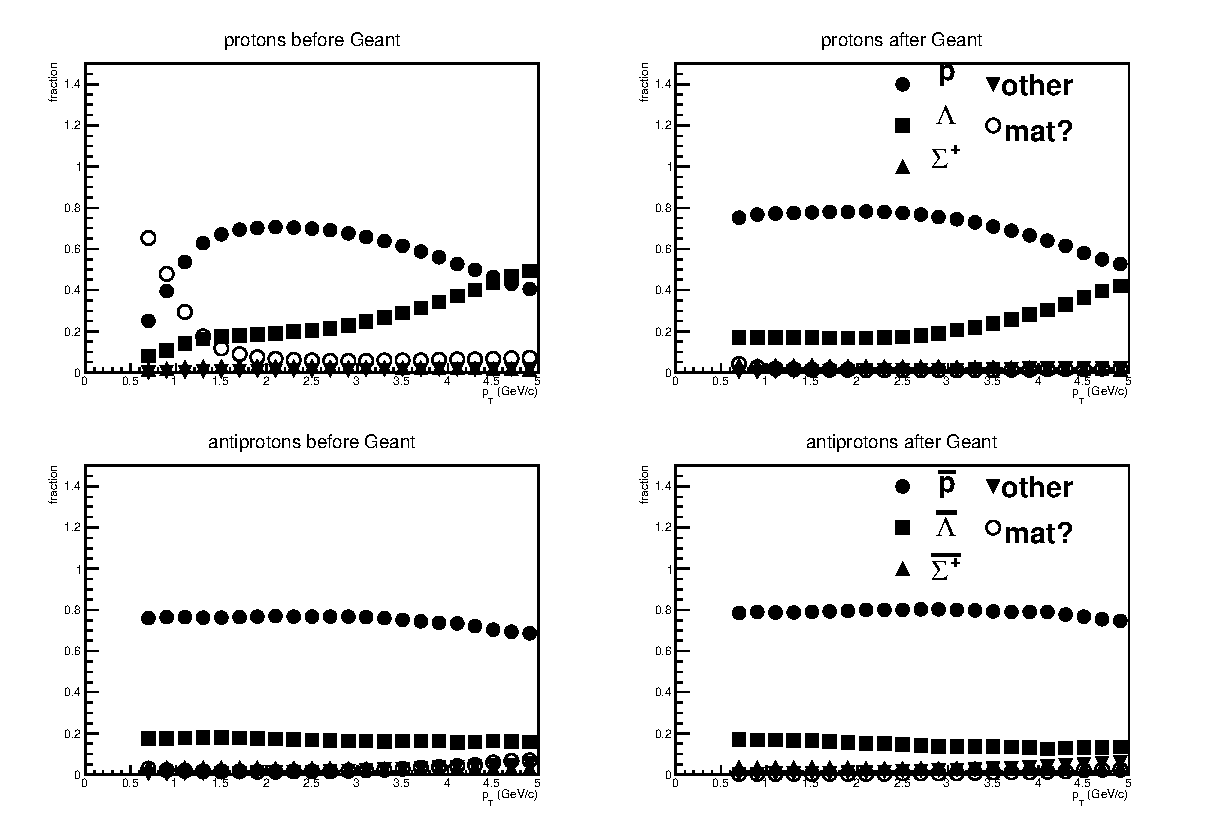
\includegraphics[width=0.99\textwidth]{pics/protonOrigin}
   \caption{Hijing p fraction}
   \label{fig:ProtonFraction}
 \end{figure}

 \begin{figure}[h!]
   \centering
   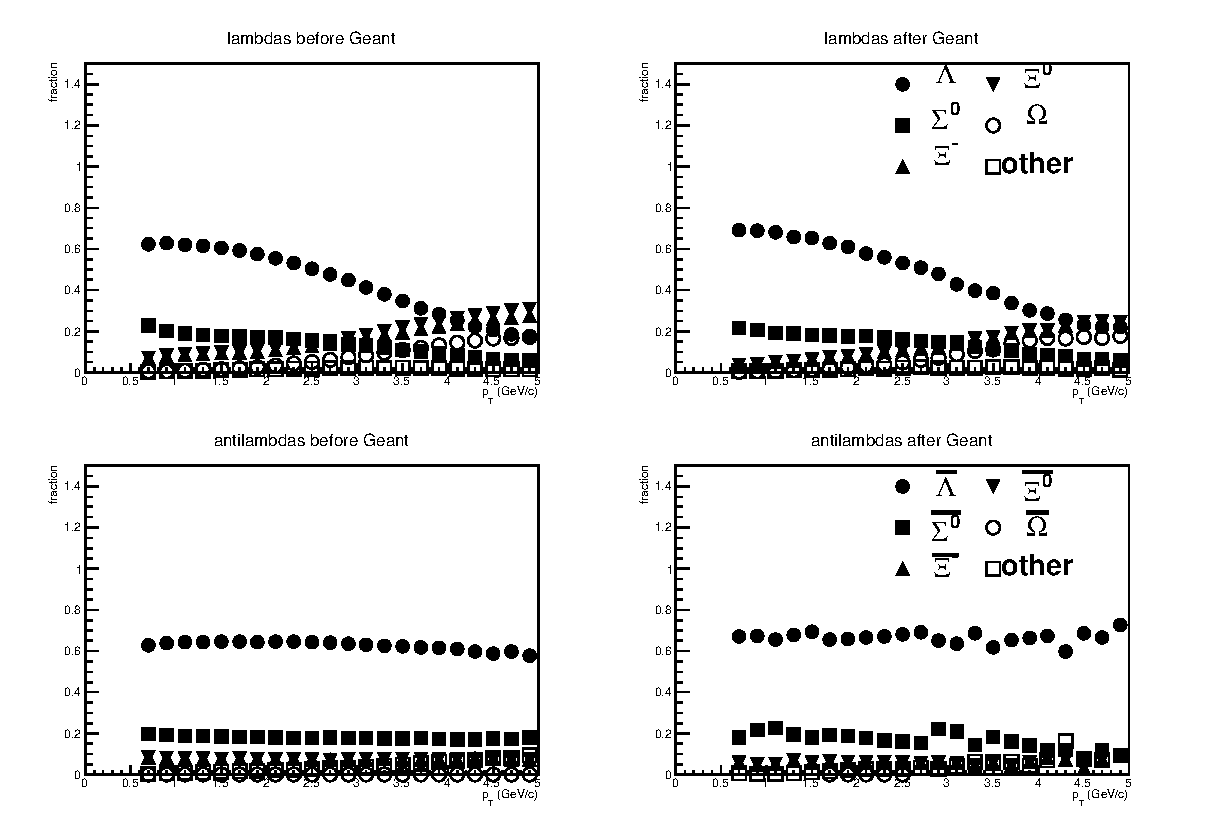
\includegraphics[width=0.99\textwidth]{pics/lambdaOrigin}
   \caption{Hijing $\Lambda$ fraction}
   \label{fig:LambdaFraction}
 \end{figure}

 \begin{figure}[h!]
   \centering
   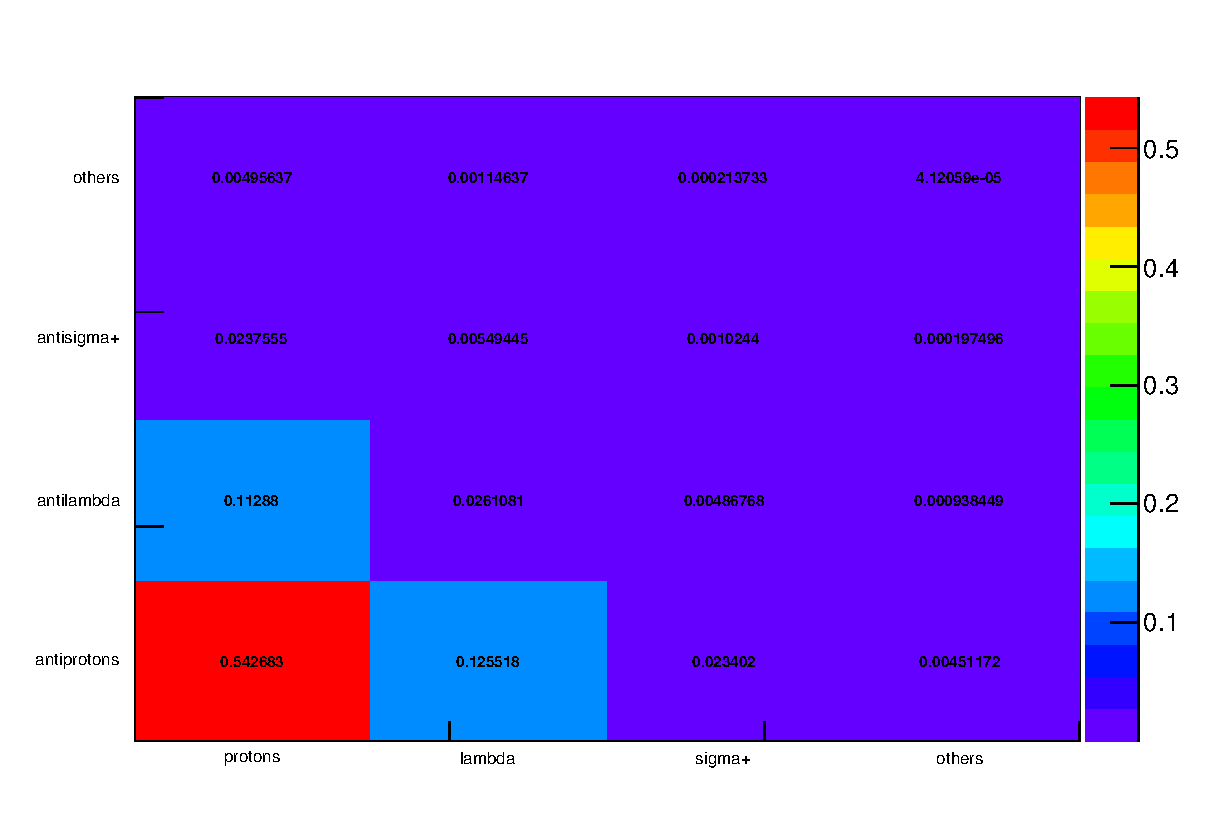
\includegraphics[width=0.99\textwidth]{pics/papFraction}
   \caption{Hijing+Geant ~\pap~Fraction $p_T$ integrated, taking into account 0.95 \p~and \ap~PID purity}
   \label{fig:papFraction}
 \end{figure}

 \begin{figure}[h!]
   \centering
   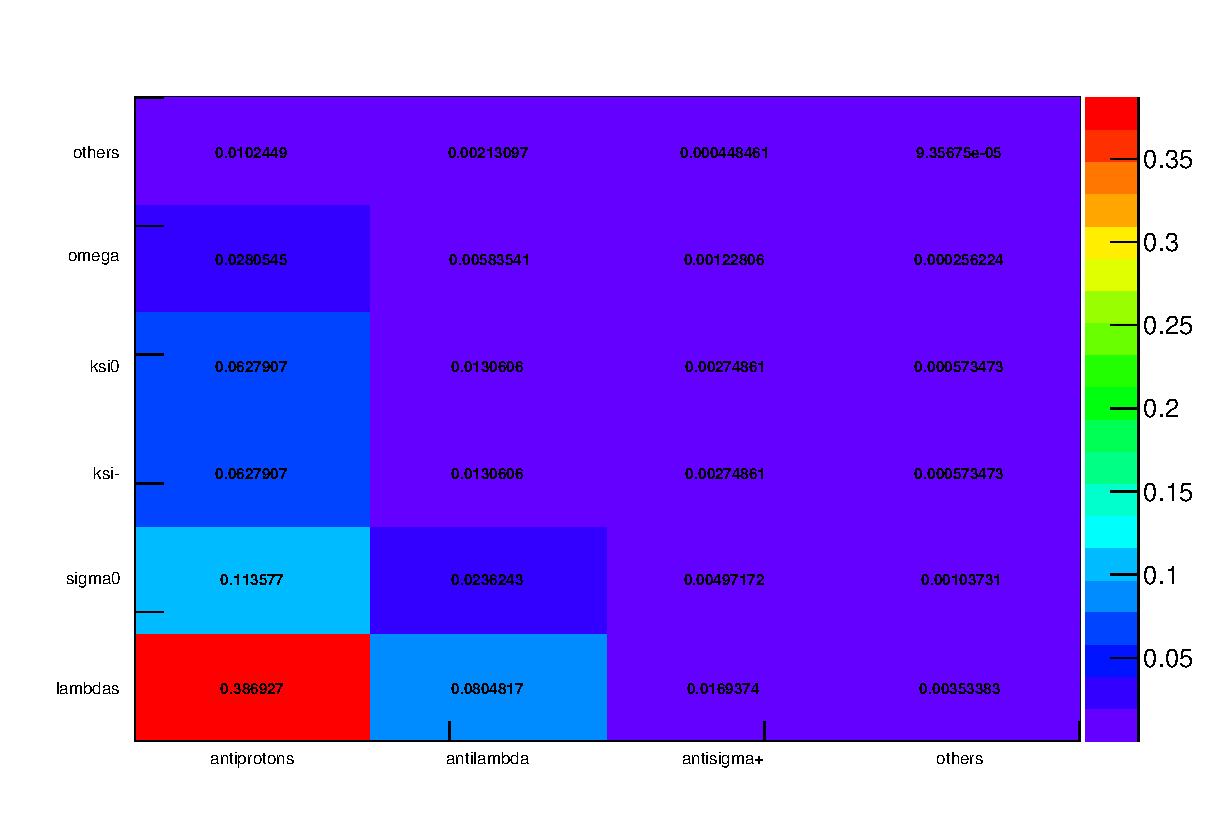
\includegraphics[width=0.99\textwidth]{pics/aplFraction}
   \caption{Hijing+Geant \apl~Fraction $p_T$ integrated, taking into account 0.95 \ap~PID purity and 0.9 $\Lambda$ purity}
   \label{fig:aplFraction}
 \end{figure}

 \begin{figure}[h!]
   \centering
   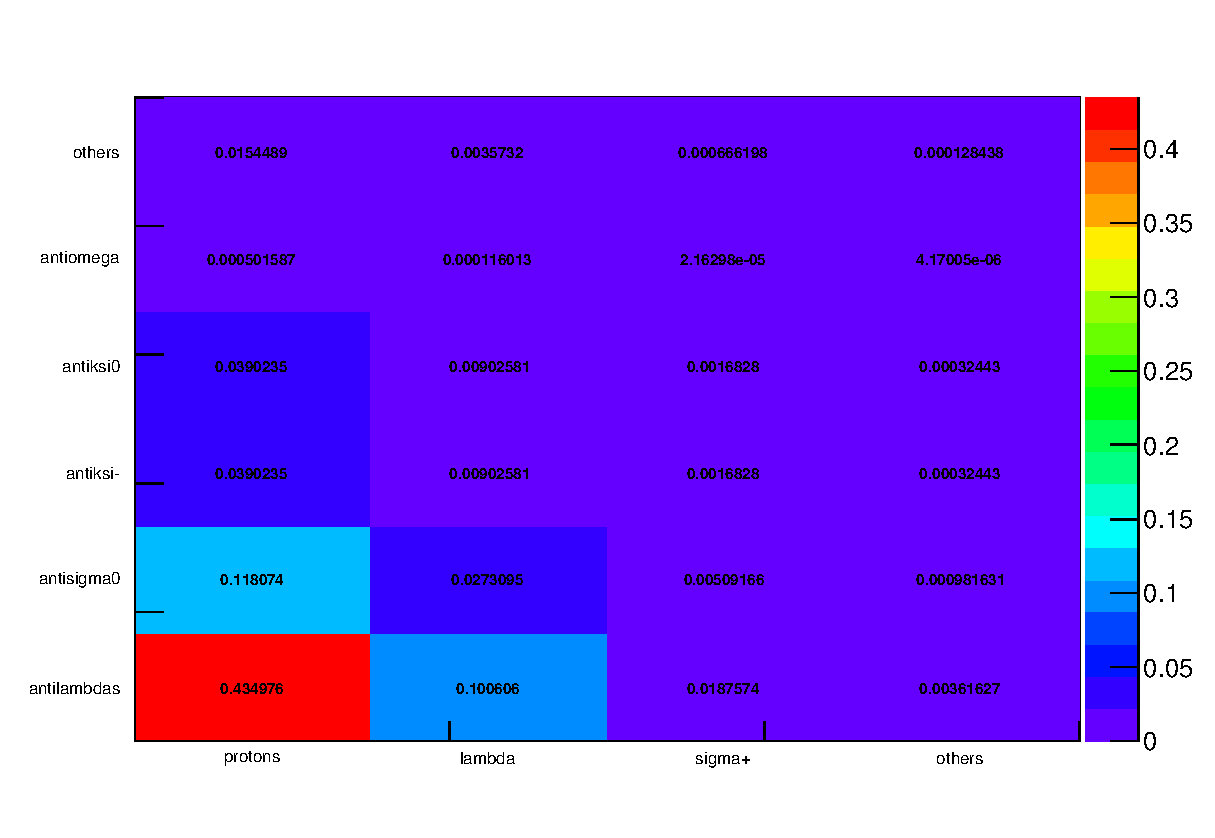
\includegraphics[width=0.99\textwidth]{pics/palFraction}
   \caption{Hijing+Geant \pal~Fraction $p_T$ integrated, 0.95 \p~PID purity and 0.9 \aL~purity}
   \label{fig:palFraction}
 \end{figure}

 \begin{figure}[h!]
   \centering
   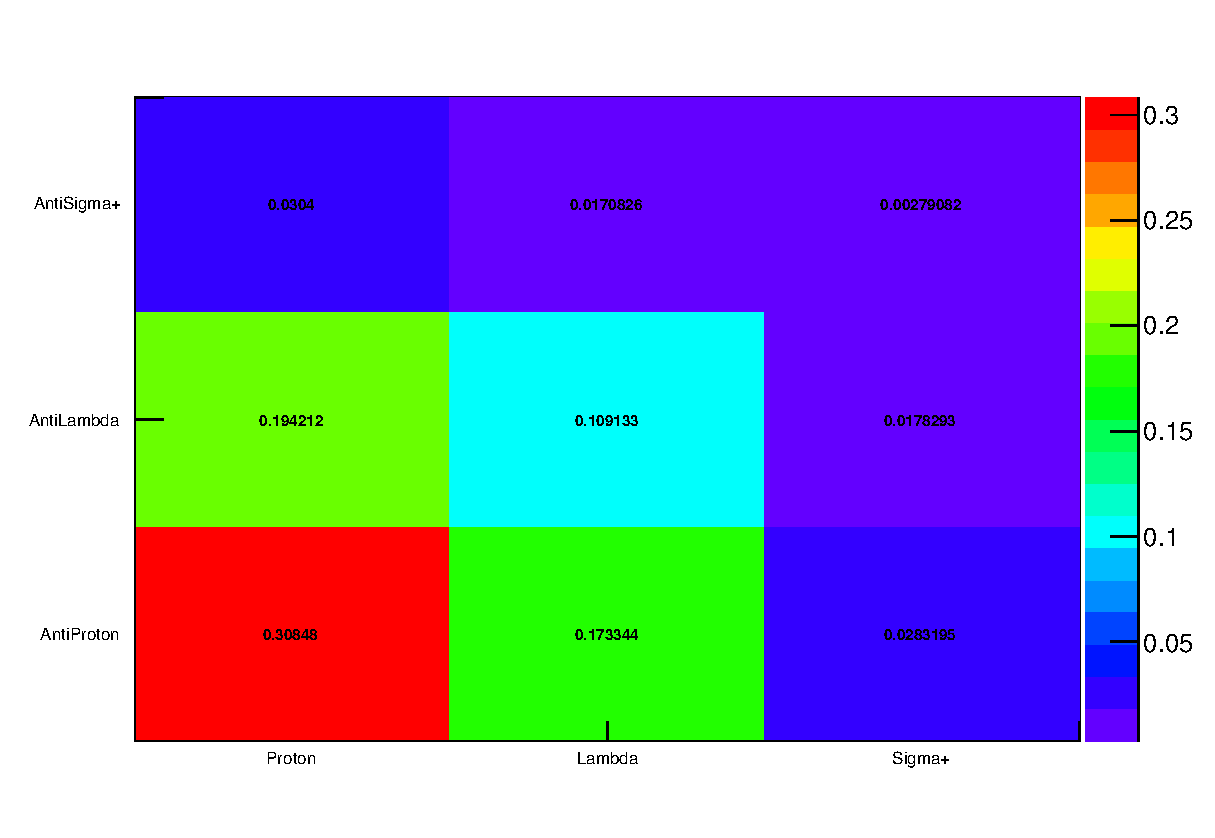
\includegraphics[width=0.99\textwidth]{pics/papFractionTherm}
   \caption{Therminator2 \pap~fraction}
   \label{fig:papFractionTherm}
 \end{figure}

  \begin{figure}[h!]
   \centering
   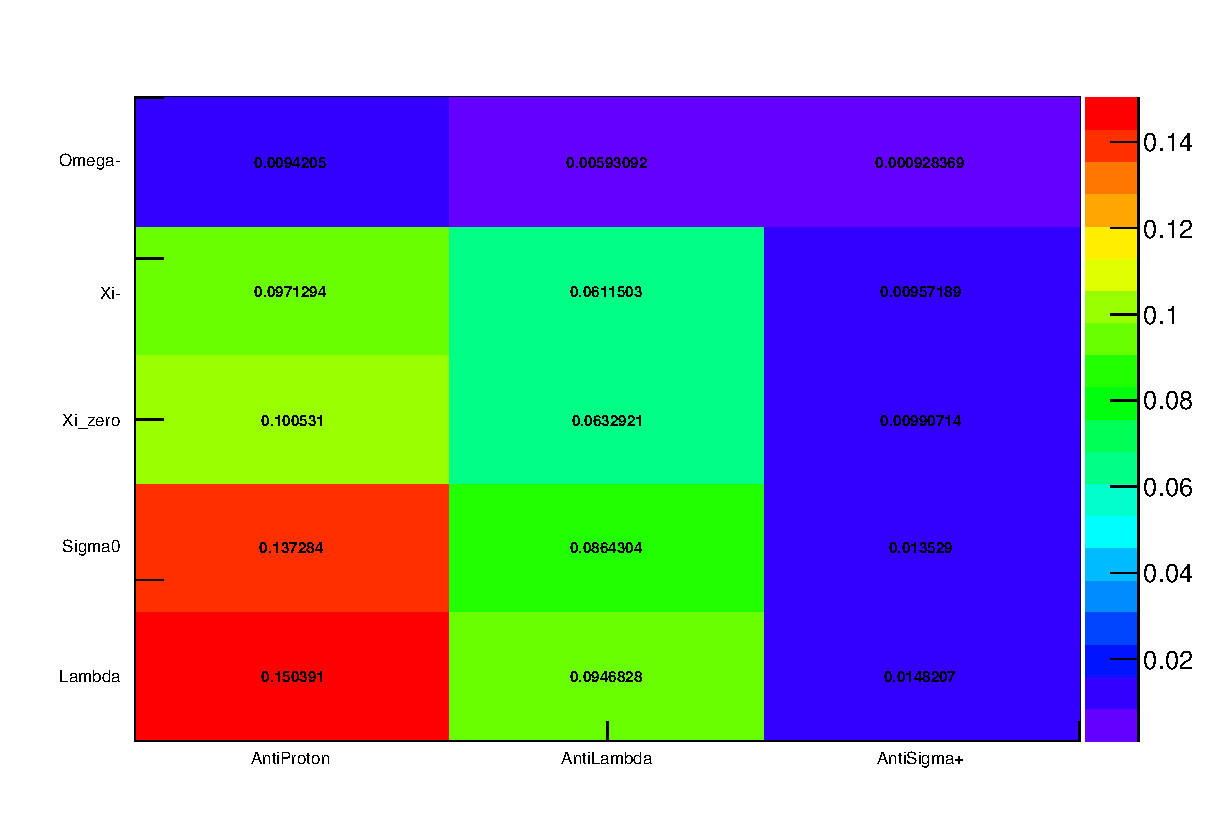
\includegraphics[width=0.99\textwidth]{pics/aplFractionTherm}
   \caption{Therminator2 \apl~fraction}
   \label{fig:aplFractionTherm}
 \end{figure}

 \begin{figure}[h!]
   \centering
   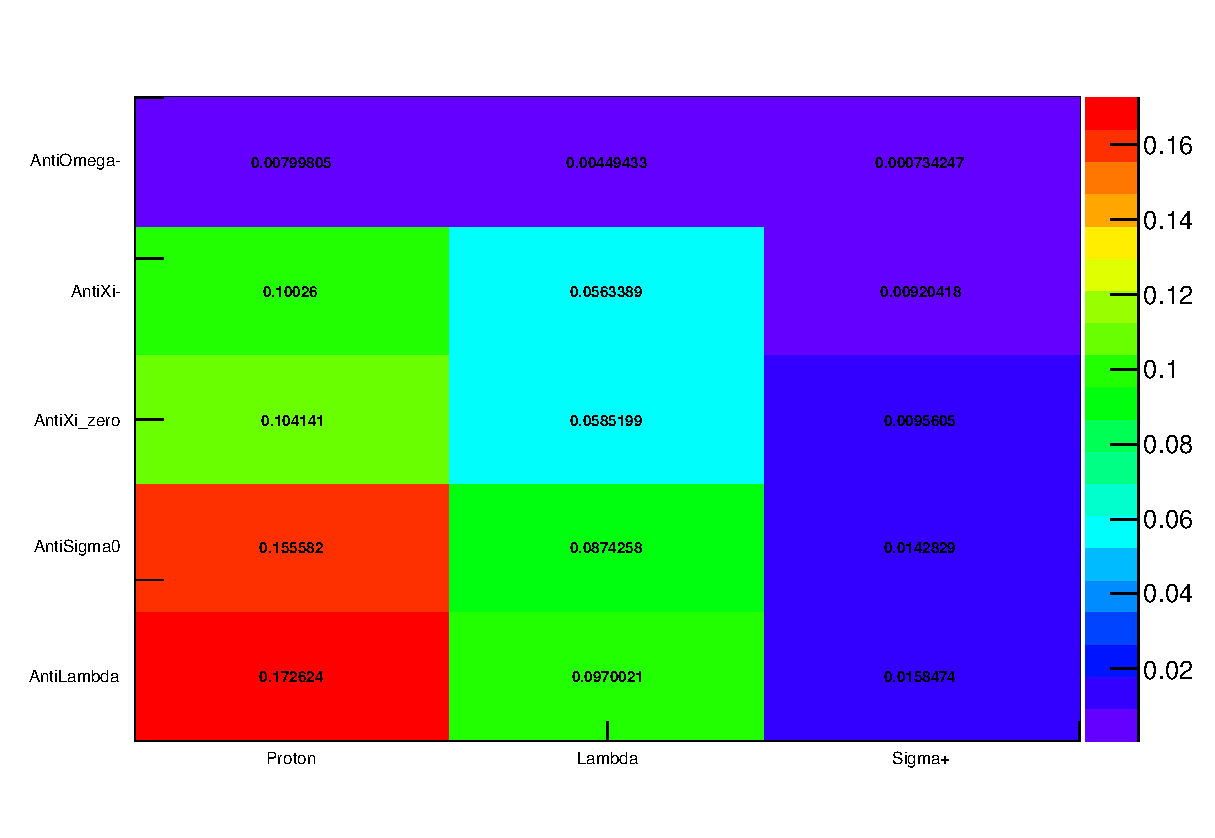
\includegraphics[width=0.99\textwidth]{pics/palFractionTherm}
   \caption{Therminator2 \pal~fraction}
   \label{fig:palFractionTherm}
 \end{figure}

%% \begin{frame}% [<+->]
%%   {\pap~fractions (Therminator)}
%%   \begin{center}
%%     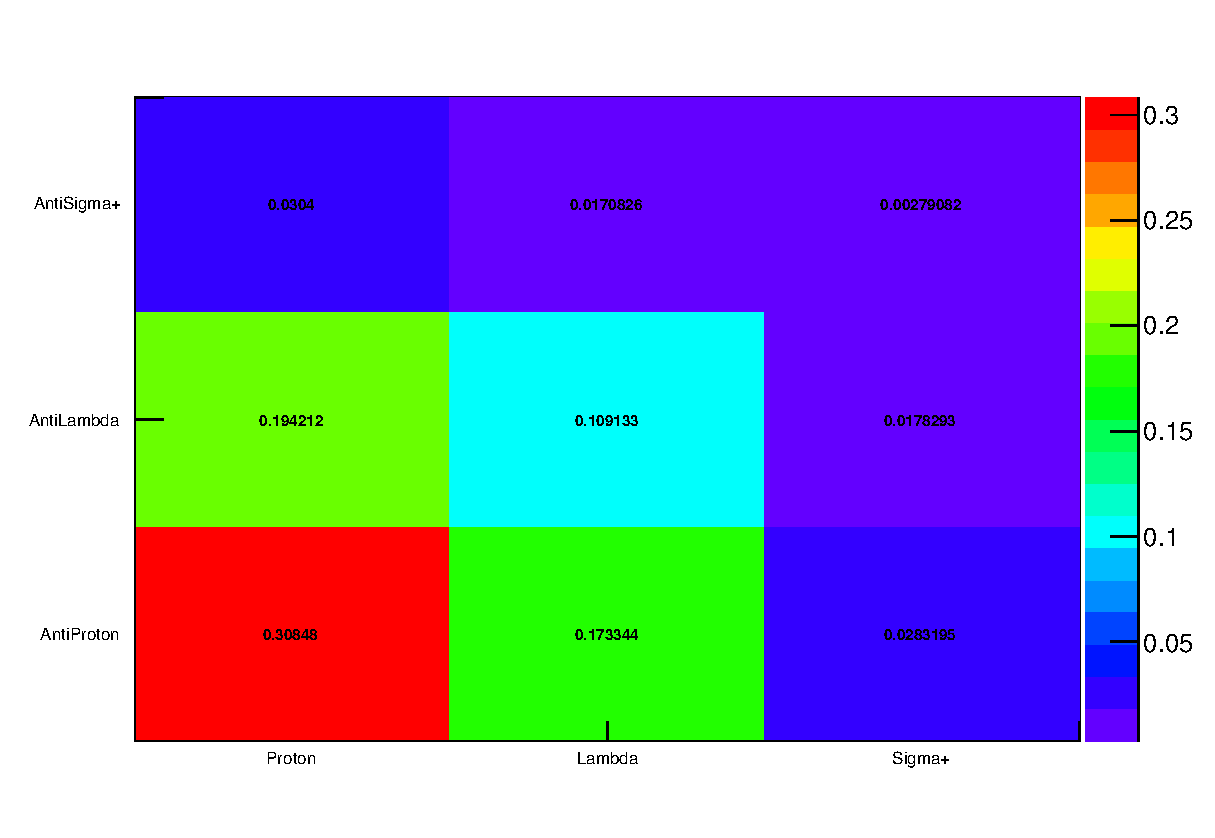
\includegraphics[width=0.9\textwidth]{pics/papFractionTherm}
%%   \end{center}
%% \end{frame}

%% \begin{frame}% [<+->]
%%   {\apl~fractions (Therminator)}
%%   \begin{center}
%%     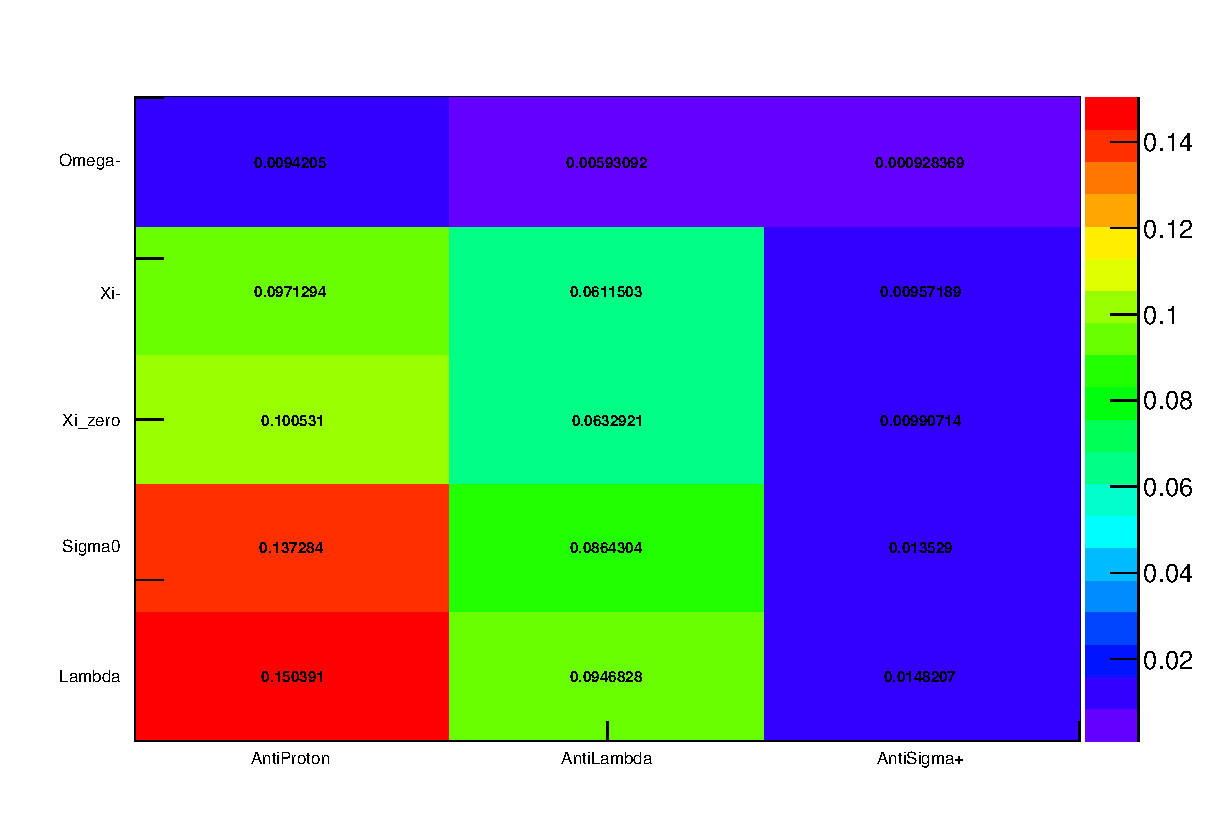
\includegraphics[width=0.9\textwidth]{pics/aplFractionTherm}
%%   \end{center}
%% \end{frame}

%% \begin{frame}% [<+->]
%%   {\pal~fractions (Therminator)}
%%   \begin{center}
%%     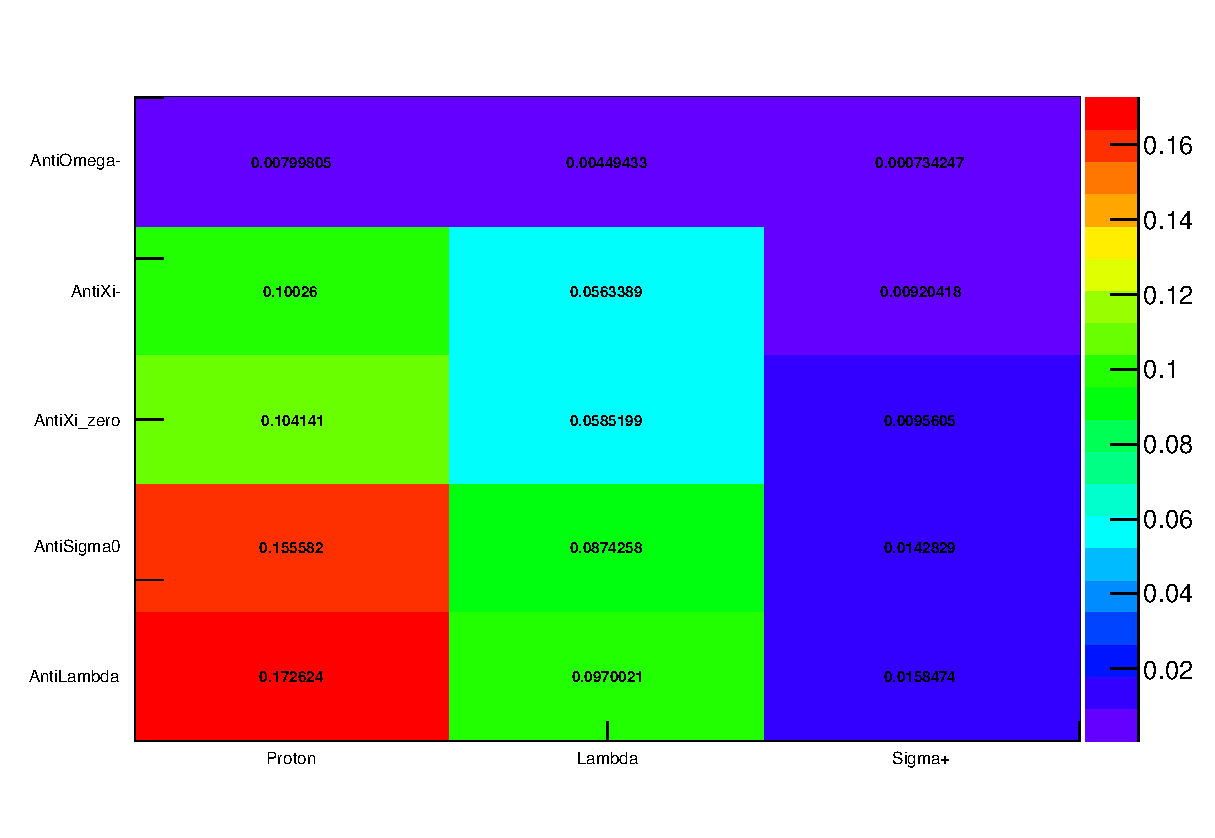
\includegraphics[width=0.9\textwidth]{pics/palFractionTherm}
%%   \end{center}
%% \end{frame}

DCA cut ?!

\section{Results}

\subsection{Correlation functions}

\begin{figure}[h!]
   \centering
   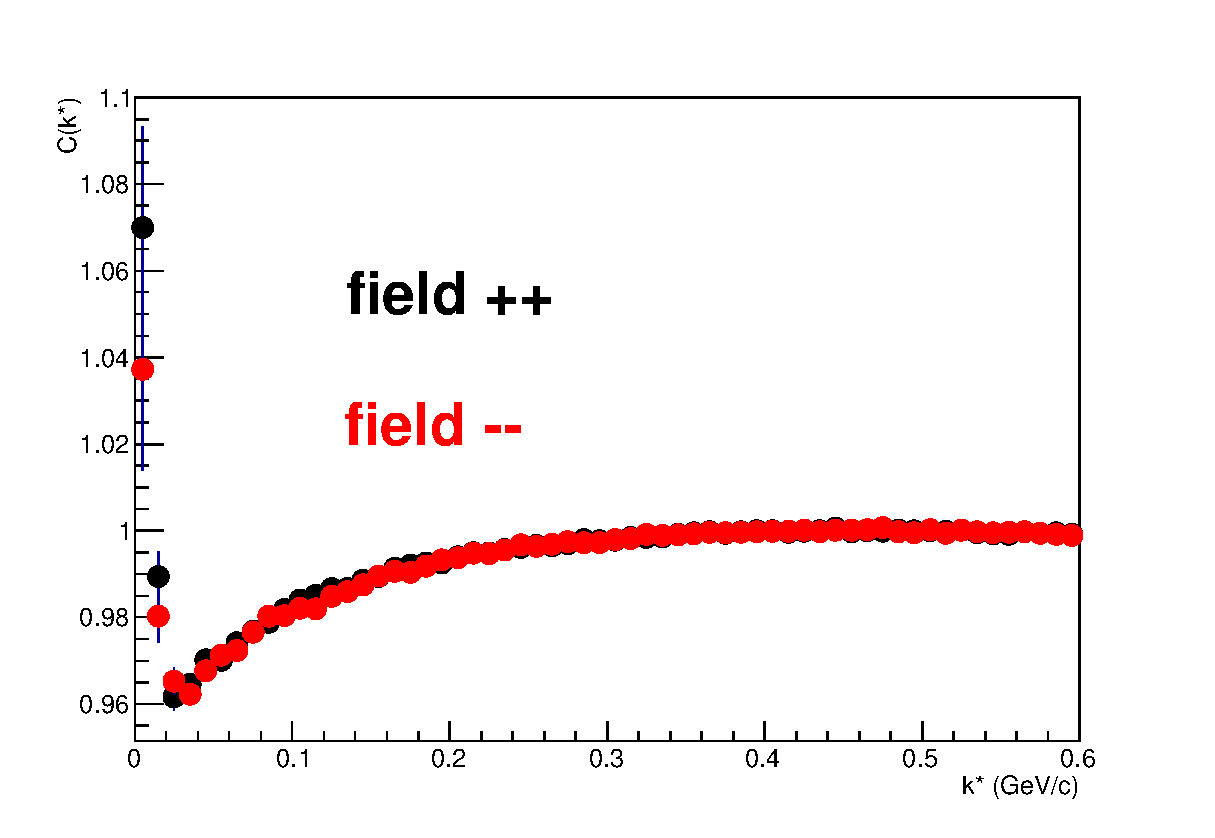
\includegraphics[width=0.99\textwidth]{pics/compPAP}
   \caption{ \pap~correlation function, centrality 0-10$\%$}
   \label{fig:papCorrFun}
 \end{figure}

\begin{figure}[h!]
   \centering
   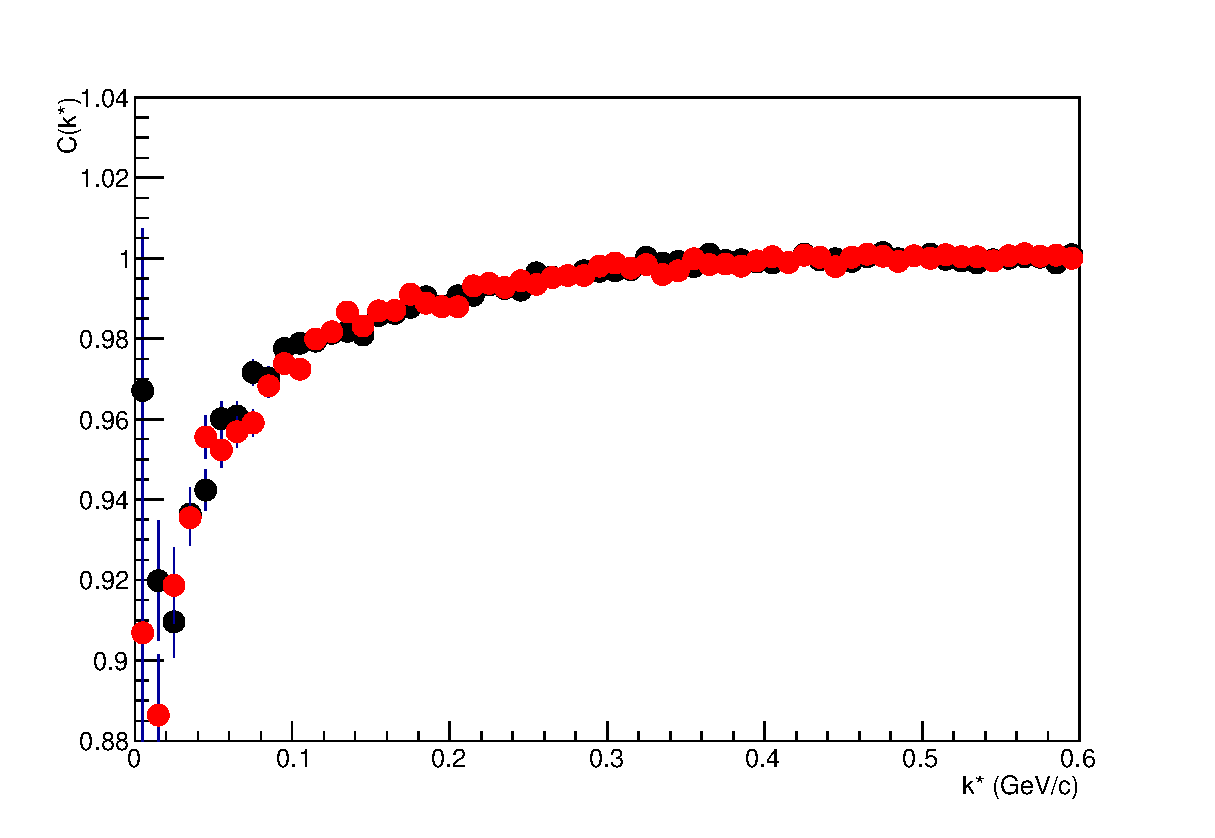
\includegraphics[width=0.99\textwidth]{pics/compPAL}
   \caption{ \pal~correlation function, centrality 0-10$\%$}
   \label{fig:palCorrFun}
 \end{figure}

\begin{figure}[h!]
   \centering
   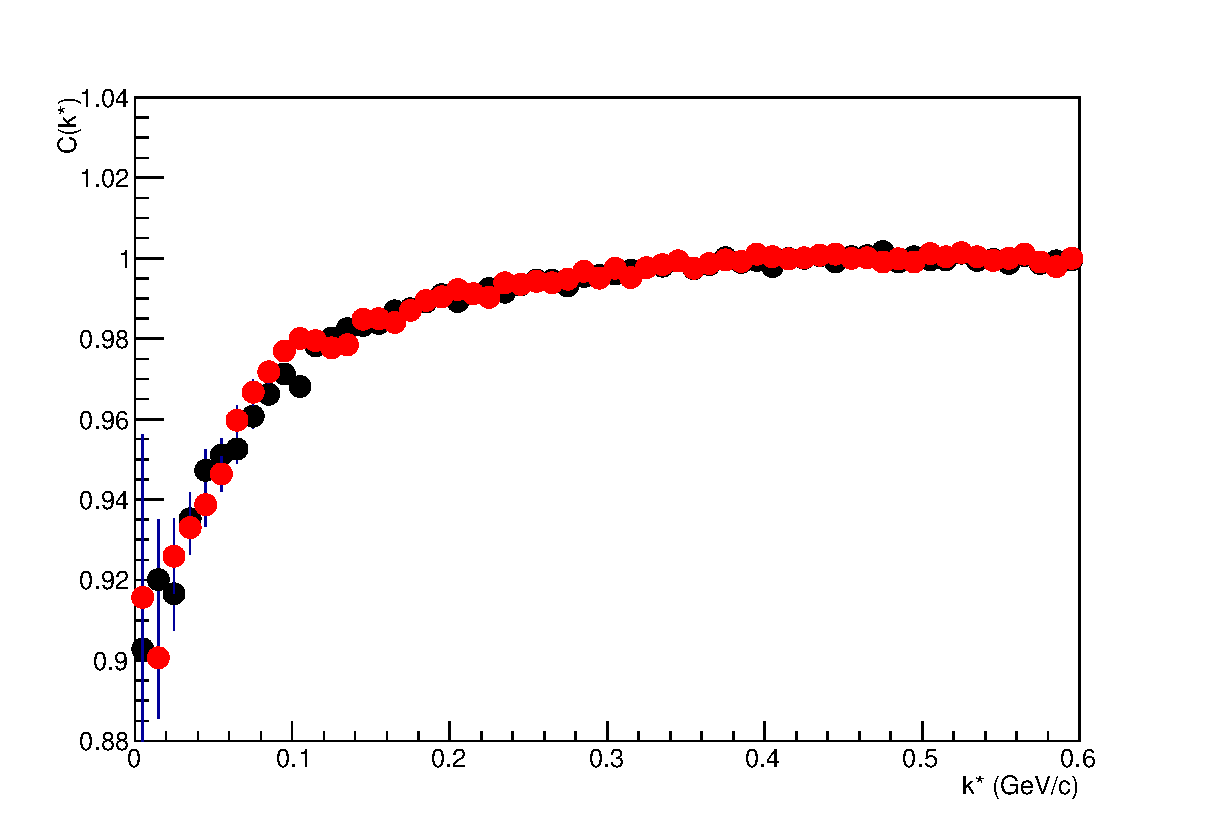
\includegraphics[width=0.99\textwidth]{pics/compAPL}
   \caption{ \apl~correlation function, centrality 0-10$\%$}
   \label{fig:aplCorrFun}
 \end{figure}

\subsection{Fitting procedure}

\subsubsection{\pap~theoretical function}

\subsection{Systematic uncertainties}
\begin{itemize}
\item non-femtoscopic background
\item fractions (Hijing vs. Therminator)
\item number of secondaries from material
\item momentum resolution correction
\item ALICE magnetic fields ++ vs. - - 
\item PID
\item different scenarios for interaction parameters
\item DCA templates
\item \pal~vs.~\apl
\item fitting procedure    
\end{itemize}

\subsubsection{Momentum resolution}
Correction for momentum resolution is taken into account in the fitting procedure. Fit function is smeared with a gaussian function with the width corresponding the momentum resolution for the pairs of interest. Following formula is used:
\begin{equation}
  C_c(q_c) = \int_{-3\sigma}^{+3\sigma}C_{th}(q_c-q) Gaus(q_t, \sigma)(q) |q_c-q|^2 d q,
\end{equation}
where $C_c$ is the corrected function, $C_{th}$ is the ideal function, $\sigma$ is the momentum resolution.

\bibliographystyle{utphys}   % Put here the style file name for the paper, i.e.apsrev4-1, utphys
\bibliography{ALICE_analysis_note}

\end{document}
